%========================================================================
%   FileName: TechNotes.tex
%     Author: GuanHWang
%      Email: GuanHWang2011@gmail.com
% LastChange: 2014-04-21 10:11:18
%========================================================================
\documentclass[10pt,technote,onecolumn,twoside]{IEEEtran}
\usepackage[CJKchecksingle,CJKnumber]{xeCJK}
\setCJKmainfont[BoldFont={SimHei},
ItalicFont={KaiTi}]{SimSun}
\renewcommand\baselinestretch{1.2}
\usepackage{graphicx}
\usepackage[usenames,dvipsnames]{xcolor}
\usepackage{listings}
\lstset{numbers=left,numbersep=4pt,
frame=lines,framerule=1pt,basicstyle=\ttfamily\scriptsize,
}
\usepackage[bookmarksnumbered, pdfencoding=auto, 
breaklinks, colorlinks, linkcolor=red, urlcolor=ForestGreen, citecolor=magenta]{hyperref}
\usepackage{cite}
\usepackage{stfloats}
\usepackage{amssymb}
\punctstyle{plain}
\begin{document}
%\begin{CJK}{UTF8}{hei}
\title{HOG/linSVM行人检测器的OpenCV实现\\技术笔记}
\author{OnceMore2020}

%Headers
\markboth{人体检测及行为分析的研究.~TechNotes.~2014}%
{GuanHao.~电子科技大学}

%Abstract
\IEEEtitleabstractindextext{%
\begin{abstract}
HOG/linSVM行人检测器在中等分辨率和低处理速度限制的应用场景下具有明显优势。HOG特征采用密集空域网格单元和重叠
的局部对比标准化来提升准确性。笔记参考Navneet Dalal和Bill Triggs在2005年的一篇CVPR文章\cite{bib1}中首次提出
HOG特征。笔记记录HOG/linSVM分类器涉及到的基本理论,并记录了使用OpenCV运算库中提供的HOG描述符实现HOG/linSVM分
类器的方法。
\end{abstract}

%Keywords
\begin{IEEEkeywords}
HOG特征,linSVM,分类器,OpenCV,行人检测,技术笔记.
\end{IEEEkeywords}}

\maketitle
\IEEEdisplaynontitleabstractindextext

\section{理论储备}
主要参考\cite{bib1},\cite{bib3},\cite{bib4}。HOG特征描述符的思想是局部对象外貌和形状等特征可以用方向梯度直方图来描述。
将图像划分为邻接的图像子区,称为单元(cell),然后对单元内的每一个像素计算方向梯度直方图,最后将这些直方图联合起来形成
最终特征。特征计算中引入了标准化操作,提升了在明亮度改变的情况下的鲁棒性。由于在局部单元上进行操作,特征对在整个空域
上发生的几何变化(只要目标保持直立行走姿势)并不敏感,使得HOG特征非常适用于人体检测。

和其它方法不同,Dalal和Triggs发现色彩和Gamma值的标准化以及高斯平滑处理在HOG特征计算中并不是必要的,并且采用了最简单的
一维离散微分模板算子。测试表明,使用Sobel算子等其它算子或是引入高斯平滑反而会造成性能降低。

\subsection{梯度矢量}
\textbf{梯度矢量(gradient vector)}是计算机视觉中的一个重要概念,许多视觉算法都需要引入对图像中每一个像素的梯度矢量的计算。
如下图显示的$3\times3$灰度图像,相应的像素标记字母作为标号。
\begin{figure*}[htbp]
\centering
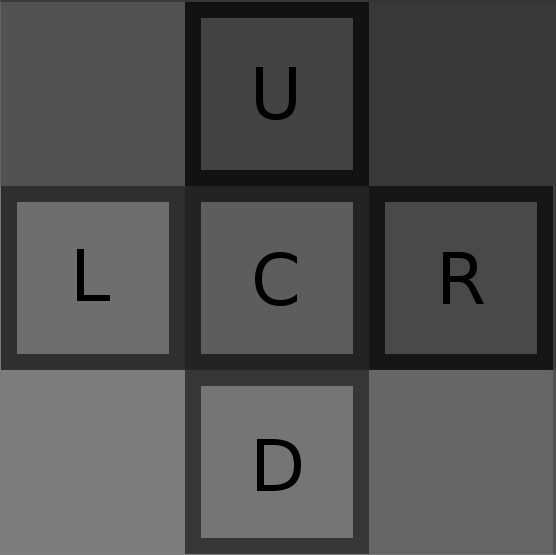
\includegraphics[width=2.2in]{gradient-3.png}
\end{figure*}

像素值在$0-255$之间,$0$表示黑色,$255$表示白色。$R-L$称为$x$方向变化率。需要注意的是,图中L像素的灰度值比R像素灰度值高,
这样计算出来会是负值,$L-R$则是正值,也称为$x$方向变化率,但是一副图像中的计算方法应当保持一致。类似的,$U-D$称为$y$方向
变化率。两个方向的变化率取值在$-255\to255$之间,不能用一个字节存储,可以映射到$0\to255$之间,这样,如果将变化率用灰度值表示,则
非常大的负变化率将映射为黑色,非常大的正变化率将映射为白色。同时,我们可以得到一个梯度矢量$[R-L,U-D]$,其幅度(magnitude)和
相角(angle)计算方法如下:
\[Magnitude=\sqrt{(R-L)^2+(U-D)^2}\]
\[Angle=arctan\left(\frac{R-L}{U-D}\right)\]

如果采用带符号梯度($-255\to255$),相角会分布在$0^\circ\to360^\circ$之间,如果采用无符号梯度(映射到$0\to255$),相角分布在
$0^\circ\to180^\circ$之间。Dalal和Triggs发现使用无符号梯度在行人检测中表现更优。

梯度矢量很好地提取了边缘信息。另一方面,试想将图像的明亮度提升,即将图像中每个像素值加上同一个常数,重新计算梯度矢量会发现
和明亮度变换之前的梯度矢量一致,这种性质使得梯度矢量可以被应用到特征提取中,即本文的人体特征提取中。
\subsection{方向梯度直方图}
如下图的一个包含行人的图像,红色框标记一个$8\times8$单元,这些$8\times8$的单元将被用来计算HOG描述符。
\begin{figure*}[!h]
\centering
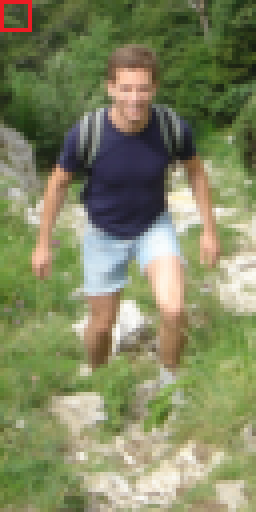
\includegraphics[width=1.6in]{hog-1.png}
\end{figure*}
在每个单元中,我们在每个像素上计算梯度矢量,将得到64个梯度矢量,梯度矢量相角在$0^\circ\to180^\circ$之间分布,我们对
相角进行分箱(bin),每箱$20^\circ$,一共9箱(Dalal和Triggs得到的最佳参数)。具有某一相角的梯度矢量的幅度按照权重分配给
直方图。这涉及到权重投票表决机制,Dalal和Triggs发现,采用梯度幅度进行分配表现最佳。例如,一个具有85度
相角的梯度矢量将其幅度的1/4分配给中心为$70^\circ$的箱,将剩余的3/4幅度分配给中心为$90^\circ$的箱。这样就得到了下面
的方向梯度直方图。
\begin{figure*}[htbp]
\centering
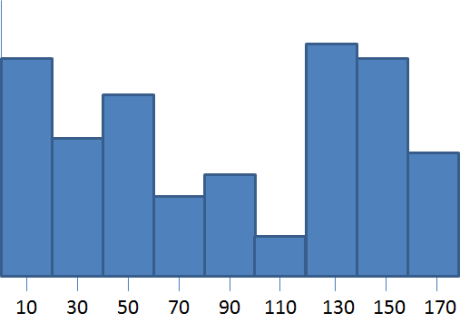
\includegraphics[width=2.5in]{hog-2.png}
\end{figure*}

上面分配幅度的方法可以减少恰好位于两箱边界的梯度矢量的影响,否则,如果一个强梯度矢量恰好在边界上,其相角的一个很小的
绕动都将对直方图造成非常大的影响。同时,在计算出梯度后进行高斯平滑,也可以缓解这种影响。

另一方面,特征的复杂程度对分类器的影响很大。通过直方图的构造,我们将特征{64个二元矢量}量化为特征{9个值},很好地压缩了
特征的同时保留了单元的信息。设想对图像加上一些失真,方向梯度直方图的变化也不会很大,这是HOG特征的优点。

前面提到,对图像所有像素进行加减后梯度矢量不变,接下来引入梯度矢量的标准化,使得其在像素值进行乘法运算后仍然保持不变。
如果对单元内的像素值都乘以某一常数,梯度矢量的幅度明显会发生变化,幅度会增加常数因子,相角保持不变,这会造成整个直方图的
每个箱的幅度增加常数因子。为了解决这个问题,需要引入梯度矢量标准化,一种简单的标准化方法是将梯度矢量除以其幅度,梯度矢量
的幅度将保持1,但是其相角不会发生变化。引入梯度矢量标准化以后,直方图各箱幅度在图像像素值整体乘以某个因子(变化对比度)时
不会发生变化。

除了对每个单元的直方图进行标准化外,另外一种方法是将固定数量的空域邻接的单元封装成区块,然后在区块上进行标准化。Dalal和Triggs使用
$2\times2$区块(50\%重叠),即$16\times16$像素。将一个区块内的四个单元的直方图信息整合为36个值的特征($9\times4$),然后对这
个36元矢量进行标准化。Dalal和Triggs考察了四种不同的区块标准化算法,设$v$为未标准化的区块梯度矢量,$||v||_k(k=1,2)$是$v$的k-范
数(norm),$e$是一个很小的常数(具体值并不重要),四种标准化算法如下:
\[L2-norm:f=\frac{v}{\sqrt{||v||^2_2+e^2}}\]
\[L2-Hys\]
\[L1-norm:f=\frac{v}{(||v||_1+e)}\]
\[L1-sqrt:f=\sqrt{\frac{v}{(||v||_1+e)}}\]
L2-Hys是在L2-norm后进行截断,然后重新进行标准化。Dalal和Triggs发现L2-Hys,L2-norm,L1-sqrt性能相似,L1-norm性能稍有下降,但
都相对于未标准化的梯度矢量有明显的性能提升。

区块重叠的影响是使得每个单元会在最终得到的HOG描述符中其作用的次数大于1次(角单元出现1次,边单元出现2次,其它单元出现4次),但
每次出现都在不同的区块进行标准化。定义一个区块位移的步长为8像素,则可以实现50\%的重叠。

如果检测器窗口为$64\time128$像素,则会被分为$7\times15$区块,每个区块包括$2\times2$个
单元,每个单元包括$8\times8$像素,每个区块进行9箱直方图统计(36值),最后的总特征矢量将有$7\times15\times4\times9=3780$个
特征值元素。

\subsection{SVM分类器}
获取了HOG特征描述符之后,需要将其递交给监督学习分类器。Dalal和Triggs使用$SVM^{light}$\cite{bib7}软件包配合HOG描述符进行
人体检测。SVM分类器寻找一个最佳超平面用作决策函数以实现二元分类,其特点是能够同时最小化经验误差与最大化几何边缘区。

\section{OpenCV实现}
OpenCV提供了采用HOG特征描述符实现的人体检测的例程:\textsf{/samples/cpp/peopledetect.cpp}。
同时提供了GPU和OPENCL加速的HOG特征描述符,分别为\textsf{gpu::HOGDescriptor}和\textsf{ocl::HOGDescriptor}。
CPU HOG的实现:\url{https://github.com/Itseez/opencv/blob/master/modules/objdetect/src/hog.cpp}
GPU加速的实现:\textsf{/samples/gpu/hog.cpp}。
OPENCL加速的实现:\textsf{/samples/ocl/hog.cpp}。

OpenCV提供的头文件在\textsf{include}文件夹中,在Ubuntu下使用源码编译OpenCV后可以在\textsf{/usr/local/include}文件夹
下找到。
\subsection{CPU HOG简单例程}
\textsf{HOGDescriptor}类定义在\textsf{object.hpp}中,一个采用\textsf{HOGDescriptor}的简单实现可以
在\url{https://github.com/Itseez/opencv/blob/master/samples/cpp/peopledetect.cpp}上找到。
程序采用了\textsf{HOGDescriptor::getDefaultPeopleDetector()}来加载默认的行人检测器,接下来的问题是怎样使用
手里已有的数据集来训练自己的分类器,这就需要了解OpenCV提供的HOG描述符类接口。

\subsection{HOGDescriptor类接口}
可以在\textsf{objdetect.hpp}中找到\textsf{HOGDescriptor}的类接口声明,
在\url{https://github.com/Itseez/opencv/blob/master/modules/objdetect/src/hog.cpp}找到其实现。但是,OpenCV没有提供
关于HOGDescriptor的文档,下面结合源码对重要的函数进行解释。

\subsubsection{HOGDescriptor::HOGDescriptor}
如下面代码所示:
\begin{lstlisting}{language=C++}
	enum { L2Hys=0 };
    enum { DEFAULT_NLEVELS=64 };

    CV_WRAP HOGDescriptor() : winSize(64,128), blockSize(16,16), blockStride(8,8),
        cellSize(8,8), nbins(9), derivAperture(1), winSigma(-1),
        histogramNormType(HOGDescriptor::L2Hys), L2HysThreshold(0.2), gammaCorrection(true),
        nlevels(HOGDescriptor::DEFAULT_NLEVELS)
    {}

    CV_WRAP HOGDescriptor(Size _winSize, Size _blockSize, Size _blockStride,
                  Size _cellSize, int _nbins, int _derivAperture=1, double _winSigma=-1,
                  int _histogramNormType=HOGDescriptor::L2Hys,
                  double _L2HysThreshold=0.2, bool _gammaCorrection=false,
                  int _nlevels=HOGDescriptor::DEFAULT_NLEVELS)
    : winSize(_winSize), blockSize(_blockSize), blockStride(_blockStride), cellSize(_cellSize),
    nbins(_nbins), derivAperture(_derivAperture), winSigma(_winSigma),
    histogramNormType(_histogramNormType), L2HysThreshold(_L2HysThreshold),
    gammaCorrection(_gammaCorrection), nlevels(_nlevels)
    {}
\end{lstlisting}
结合理论基础,很容易理解其参数列表:
\begin{enumerate}
\item[$\bullet$]\textbf{\_winSize}~~检测器窗口尺寸,需要和区块尺寸和区块步进对齐。默认采用$64\times128$像素。
\item[$\bullet$]\textbf{\_blockSize}~~区块尺寸,需要和单元尺寸对齐。默认采用$16\times16$像素。
\item[$\bullet$]\textbf{\_blockStride}~~区块步进,需要是单元尺寸的整数倍。默认采用$8\times8$像素。
\item[$\bullet$]\textbf{\_cellSize}~~单元尺寸。默认采用$8\times8$像素。
\item[$\bullet$]\textbf{\_nbins}~~分箱数量。默认采用9箱。
\item[$\bullet$]\textbf{\_derivAperture}~~微分算子。
\item[$\bullet$]\textbf{\_winSigma}~~高斯平滑窗口参数。
\item[$\bullet$]\textbf{\_histogramNormType}~~直方图标准化方式。默认采用L2-Hys标准化\cite{bib5}。
\item[$\bullet$]\textbf{\_L2HysThreshold}~~L2-Hys标准化截断门限值。默认采用0.2。
\item[$\bullet$]\textbf{\_gammaCorrection}~~标识是否要加入伽玛校正预处理模块。默认采用。
\item[$\bullet$]\textbf{\_nlevels}~~多尺寸检测时HOG检测窗口最大缩放倍数。默认为64。
\end{enumerate}
其中\textsf{nlevels}变量需要结合\textsf{hog.cpp}中的下面代码来理解其意思:
\begin{lstlisting}{language=C++}
for( levels = 0; levels < nlevels; levels++ )
{
	levelScale.push_back(scale);
    if( cvRound(imgSize.width/scale) < winSize.width ||
        cvRound(imgSize.height/scale) < winSize.height ||
        scale0 <= 1 )
            break;
        scale *= scale0;
}
\end{lstlisting}

\subsubsection{HOGDescriptor::getDescriptorSize}
返回HOG特征描述符维度。
\subsubsection{HOGDescriptor::setSVMDetector}
设置线性SVM分类器的参数。
\subsubsection{HOGDescriptor::getDefaultPeopleDetector}
返回OpenCV提供的用于人体检测的分类器参数(默认检测器窗口尺寸)。
\subsubsection{HOGDescriptor::detect}
进行对象检测,不进行检测窗口多尺寸缩放。
\begin{lstlisting}{language=C++}
HOGDescriptor::detect(const Mat& img, CV_OUT std::vector<Point>& foundLocations,
                        CV_OUT std::vector<double>& weights,
                        double hitThreshold = 0, Size winStride = Size(),
                        Size padding = Size(),
                        const std::vector<Point>& searchLocations = std::vector<Point>())
\end{lstlisting}
参数列表:
\begin{enumerate}
\item[$\bullet$]\textbf{img}~~图像源文件,目前支持\textsf{CV\_8UC1}和\textsf{CV\_8UC4}格式的图像。
\item[$\bullet$]\textbf{foundLocations}~~检测到的目标对象边界左上角点的位置。
\item[$\bullet$]\textbf{weights}~~检测到的目标的可信度。
\item[$\bullet$]\textbf{hitThreshold}~~SVM分类判定平面之间的距离门限。默认为0。
\item[$\bullet$]\textbf{winStride}~~窗口步进,需要是区块步进的整数倍。
\item[$\bullet$]\textbf{padding}~~图像边框尺寸
\item[$\bullet$]\textbf{searchLocations}~~划窗方法当前所在位置的边界左上角点的位置
\end{enumerate}
程序先计算当前窗口的HOG特征描述符,然后计算距离,再与\textsf{hitThreshold}进行比较,如果大于\textsf{hitThreshold}
则存进\textsf{foundLocations}。
\subsubsection{HOGDescriptor::detectMultiScale}
进行多尺寸窗口目标对象检测。要检测多尺寸的目标,有两种方法:一是图像尺寸不变,缩放检测窗口大小,二是检测窗口不变,
缩放图像尺寸。
\begin{lstlisting}{language=C++}
HOGDescriptor::detectMultiScale(const Mat& img, CV_OUT vector<Rect>& foundLocations,
                                  CV_OUT vector<double>& foundWeights, double hitThreshold=0,
                                  Size winStride=Size(), Size padding=Size(), double scale=1.05,
                                  double finalThreshold=2.0,bool useMeanshiftGrouping = false)
\end{lstlisting}
与\textsf{HOGDescriptor::detect}相比增加的参数解释:
\begin{enumerate}
\item[$\bullet$]\textbf{scale}~~每次缩放的比例
\item[$\bullet$]\textbf{finalThreshold}~~聚类筛选门限
\item[$\bullet$]\textbf{useMeanshiftGrouping}~~聚类方法
\end{enumerate}
结合下面的源码:
\begin{lstlisting}{language=C++}
for( levels = 0; levels < nlevels; levels++ )
{
	levelScale.push_back(scale);
    if( cvRound(imgSize.width/scale) < winSize.width ||
        cvRound(imgSize.height/scale) < winSize.height ||
        scale0 <= 1 )
            break;
        scale *= scale0;
}
\end{lstlisting}
可知\textsf{HOGDescriptor::detectMultiScale}采用的是第二种方法。当图像缩小到比检测窗口小的时候就不再
进行缩放了。

当检测结束时,一些对象可能会被多个矩形窗口包围(检测到),需要对这些窗口进行聚类分析。
\begin{lstlisting}{language=C++}
if ( useMeanshiftGrouping )
        groupRectangles_meanshift(foundLocations, foundWeights, foundScales, finalThreshold, winSize);
    else
        groupRectangles(foundLocations, foundWeights, (int)finalThreshold, 0.2);
\end{lstlisting}
当\textsf{useMeanshiftGrouping}为\textsf{true}时,调用\textsf{groupRectangle\_meanshift}进行聚类,
否则调用\textsf{groupRectangle}进行聚类(默认采用)。\textsf{groupRectangle}函数对所有输入矩形采用
矩形相似标准(相似尺寸和位置)进行聚类,最后一个参数0.2表示聚类时的相似度判决参数。然后某些些矩形类内
矩形数量小于等于\textsf{finalThreshold}的矩形类被排除。然后将输出存进\textsf{foundLocations}。

\subsubsection{HOGDescriptor::compute}
返回对整个图像计算得到的HOG描述符。用于分类器的训练。
\begin{lstlisting}{language=C++}
HOGDescriptor::compute(const Mat& img,
                         CV_OUT vector<float>& descriptors,
                         Size winStride=Size(), Size padding=Size(),
                         const std::vector<Point>& locations=std::vector<Point>())
\end{lstlisting}
参数列表:
\begin{enumerate}
\item[$\bullet$]\textbf{img}~~源文件
\item[$\bullet$]\textbf{descriptors}~~存储HOG描述符
\item[$\bullet$]\textbf{locations}~~
\end{enumerate}

\subsection{HOG/linSVM程序实现}
在$SVM^{Light}$网站上可以下载到其程序包,将解压缩的文件放到文件夹\textsf{svmlight}当中。实现过程参考\cite{bib8}。
\subsubsection{训练HOG描述符}
在工作目录下设置文件夹\textsf{/pos}和\textsf{/neg}分别用于放置阳性样本和阴性样本。

代码:\url{https://gist.github.com/OnceMore2020/11162992}
% text color
%\textcolor{teal}{}

%lstling env
%\begin{lstlisting}[language=bash]
%
%\end{lstlisting}

%Single Column Floating Figure
%\begin{figure*}[!t]
%\centering
%\includegraphics[width=5in]{myfigure.pdf}
%\caption{Simulation Results.}
%\label{fig_sim}
%\end{figure*}

%double column floating figure
%\begin{figure*}[!t]
%\centering
%\subfloat[Case I]{\includegraphics[width=2.5in]{box}%
%\label{fig_first_case}}
%\hfil
%\subfloat[Case II]{\includegraphics[width=2.5in]{box}%
%\label{fig_second_case}}
%\caption{Simulation results.}
%\label{fig_sim}
%\end{figure*}

%Floating Table
%\begin{table}[!t]
%\renewcommand{\arraystretch}{1.3}
%\caption{An Example of a Table}
%\label{table_example}
%\centering
%\begin{tabular}{|c||c|}
%\hline
%One & Two\\
%\hline
%Three & Four\\
%\hline
%\end{tabular}
%\end{table}


% bibliography section
\begin{thebibliography}{99}
\bibitem{bib1}
N. Dalal and B. Triggs, “Histograms of Oriented Gradients for
Human Detection,” Proc. IEEE Int’l Conf. Computer Vision and
Pattern Recognition, pp. 886-893, 2005.
\bibitem{bib2}
Object Detection,\url{http://docs.opencv.org/modules/gpu/doc/object_detection.html}
\bibitem{bib3}
HOG PERSON DETECTOR TUTORIAL,\url{http://chrisjmccormick.wordpress.com/2013/05/09/hog-person-detector-tutorial/}
\bibitem{bib4}
GRADIENT VECTORS,\url{http://chrisjmccormick.wordpress.com/2013/05/07/gradient-vectors/}
\bibitem{bib5}
D.G.Lowe.Distinctive image features from scale-invariant keypoints.IJCV,2004.
\bibitem{bib6}
Histogram of oriented gradients,\url{http://en.wikipedia.org/wiki/Histogram_of_oriented_gradients}
\bibitem{bib7}
SVMLight,Support Vector Machine,\url{http://svmlight.joachims.org/}
\bibitem{bib8}
trainHOG,\url{https://github.com/DaHoC/trainHOG}
\bibitem{bib9}
Improving Object Detection with Boosted Histograms,I. Laptev; in Proc. BMVC'06, Edinburgh, UK, pp. III:949-958.
\end{thebibliography}
%
%\end{IEEEbiography}
%\end{CJK}
\end{document}
